\documentclass{beamer}

\AtBeginSubsection[]
{
\begin{frame}<beamer>
\frametitle{Plan}
\tableofcontents[
  currentsection,
  sectionstyle=show/hide,
  subsectionstyle=show/shaded/hide
]
\end{frame}
}

\usepackage[francais]{babel}
\usepackage[utf8x]{inputenc}
\usepackage[T1]{fontenc}
\usepackage{listings}

\mode<presentation> {

% The Beamer class comes with a number of default slide themes
% which change the colors and layouts of slides. Below this is a list
% of all the themes, uncomment each in turn to see what they look like.

%\usetheme{default}
%\usetheme{AnnArbor}
%\usetheme{Antibes}
%\usetheme{Bergen}
%\usetheme{Berkeley}
%\usetheme{Berlin}
%\usetheme{Boadilla}
%\usetheme{CambridgeUS}
%\usetheme{Copenhagen}
%\usetheme{Darmstadt}
%\usetheme{Dresden}
%\usetheme{Frankfurt}
%\usetheme{Goettingen}
%\usetheme{Hannover}
%\usetheme{Ilmenau}
%\usetheme{JuanLesPins}
%\usetheme{Luebeck}
\usetheme{Madrid}
%\usetheme{Malmoe}
%\usetheme{Marburg}
%\usetheme{Montpellier}
%\usetheme{PaloAlto}
%\usetheme{Pittsburgh}
%\usetheme{Rochester}
%\usetheme{Singapore}
%\usetheme{Szeged}
%\usetheme{Warsaw}

% As well as themes, the Beamer class has a number of color themes
% for any slide theme. Uncomment each of these in turn to see how it
% changes the colors of your current slide theme.

%\usecolortheme{albatross}
%\usecolortheme{beaver}
%\usecolortheme{beetle}
%\usecolortheme{crane}
%\usecolortheme{dolphin}
%\usecolortheme{dove}
%\usecolortheme{fly}
%\usecolortheme{lily}
%\usecolortheme{orchid}
%\usecolortheme{rose}
%\usecolortheme{seagull}
%\usecolortheme{seahorse}
%\usecolortheme{whale}
%\usecolortheme{wolverine}

%\setbeamertemplate{footline} % To remove the footer line in all slides uncomment this line
%\setbeamertemplate{footline}[page number] % To replace the footer line in all slides with a simple slide count uncomment this line

%\setbeamertemplate{navigation symbols}{} % To remove the navigation symbols from the bottom of all slides uncomment this line
}

\usepackage{graphicx}
\graphicspath{ {img/} }
\usepackage{booktabs}
\newsavebox{\longestsec}% Box to save longest sectional heading
\title[Exploitation binaire]{Exploitation binaire : Une introduction (1/2)}

\author{Frédéric Vachon}
 
\date{\today}

\begin{document}

\begin{frame}
\titlepage
\end{frame}

\begin{frame}[plain,c]
\frametitle{Plan de la présentation}
\tableofcontents
\end{frame}


%--------------------------------------
%  ASSEMBLEUR x86
%--------------------------------------
\section{Assembleur x86}

%--------------------------------------
\subsection{Mémoire}

\begin{frame}{\insertsection: \insertsubsection}
  \centering
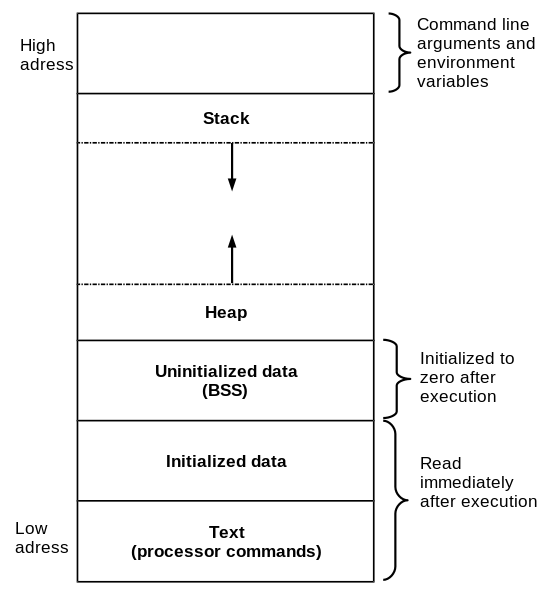
\includegraphics[scale=0.35]{memlayout}
\end{frame}

%--------------------------------------
\subsection{Registres}

\begin{frame}{\insertsection: \insertsubsection}
  \begin{itemize}
  \item Registres généraux
    \begin{itemize}
    \item EAX, EBX, ECX, EDX, ESI, EDI
    \item EAX => AX, AH, AL
    \end{itemize}
  \item Registres pour la pile
    \begin{itemize}
    \item ESP : Pointeur de pile
    \item EBP : Pointeur de base de pile
    \end{itemize}
  \item Pointeur d'instructions
    \begin{itemize}
    \item EIP
    \end{itemize}
  \end{itemize}


\end{frame}

%--------------------------------------
\subsection{Instructions}


% SLIDE 1
\begin{frame}{\insertsection: \insertsubsection}
  \begin{itemize}
  \item Syntaxe Intel
  \item Déplacement de données
    \begin{block}{MOV}
        MOV EAX, 0x41414141 // Met 0x41414141 dans EAX\\
        MOV EAX, [EDI] // Met la valeur pointée par EDI dans EAX
    \end{block}
    \begin{block}{LEA}
      LEA EAX, [EAX+1] // EAX = EAX + 1
    \end{block}
  \end{itemize}
\end{frame}


% SLIDE 2
\begin{frame}{\insertsection: \insertsubsection}
  \begin{itemize}
  \item Manipulation de la pile
    \begin{block}{Ajout d'une valeur sur la pile}
      PUSH EAX // RSP += 4; *RSP = EAX;
    \end{block}
    \begin{block}{Retrait d'une valeur sur la pile}
      POP EAX // EAX = *RSP; RSP -= 4;
    \end{block}
  \end{itemize}
\end{frame}

% SLIDE 3
\begin{frame}{\insertsection: \insertsubsection}
  \begin{itemize}
  \item Arithmétique de base
    \begin{block}{Arithmétique}
      ADD EAX, EBX\\
      SUB EBX, 0x2\\
      SUB AL, BL\\
      INC EDX\\
      DEC ECX\\
    \end{block}
  \end{itemize}
\end{frame}

% SLIDE 3
\begin{frame}{\insertsection: \insertsubsection}
  \begin{block}{Appel de fonctions}
    CALL 0x0804010\\
    CALL EAX\\
    CALL [EAX]
  \end{block}
  \begin{block}{Retour d'une fonction}
    RET
  \end{block}
\end{frame}

% SLIDE 3
\begin{frame}{\insertsection: \insertsubsection}
  \begin{block}{Comparaison}
    CMP EAX, EBX\\
    TEST EAX, EAX // Si EAX = 0, ZF = 1
  \end{block}
  \begin{block}{Sauts conditionnels}
    JZ 0x0804010 // Saute si les deux valeurs sont égales\\
    JE 0x0804010 // Saute si les deux valeurs sont égales\\
    JNZ 0x0804010 // Saute si les deux valeurs ne sont pas égales\\
    JNE 0x0804010 // Saute si les deux valeurs ne sont pas égales\\
  \end{block}
\end{frame}


%--------------------------------------
%  DU C VERS L'ASSEMBLEUR
%--------------------------------------
\section{Du C vers l'assembleur}

\subsection{Cadres d'activation (stack frame)}

\subsection{Appels de fonctions}

\subsection{Conditions}


%--------------------------------------
%  BUFFER OVERFLOW ET EXPLOITATION
%--------------------------------------
\section{Buffer overflow et Exploitation}
\subsection{Fonctions vulnérables}
\subsection{Changer une variable sur la pile}
\subsection{Contrôler l'adresse de retour}
\subsection{Injection et exécution d'un shellcode}

\section{Débogguage Bas Niveau}

\begin{frame}
  salut
\end{frame}


\end{document}